\documentclass[aspectratio=169]{beamer}

% Theme
\usetheme{metropolis}
\setbeamertemplate{navigation symbols}{}

% Packages
\usepackage{amsmath}
\usepackage{amssymb}
\usepackage{graphicx}
\usepackage{booktabs}
\usepackage{xcolor}
\usepackage{array}

% Custom colors
\definecolor{alertred}{RGB}{231, 76, 60}
\definecolor{successgreen}{RGB}{46, 204, 113}

% Title information
\title{Do Protests Really Spread?}
\subtitle{Self-Excitation in Indonesian Protests}
\author{Daniel Carnahan}
\date{January 2026}
\institute{}

\begin{document}

% =============================================================================
% TITLE SLIDE
% =============================================================================

\maketitle

% =============================================================================
% SECTION 1: MOTIVATION
% =============================================================================

\section{Motivation}

% -----------------------------------------------------------------------------
\begin{frame}{Research Question}

\textbf{Central question:} Do protests really spread?

\vspace{1em}

Scholars have long studied protest waves and diffusion, but a key puzzle remains:

\begin{itemize}
    \item Does observed clustering reflect \textit{true contagion}---protests causing protests?
    \item Or \textit{common shocks}---independent responses to shared conditions?
\end{itemize}

\vspace{1em}

\textbf{Two sub-questions:}

\begin{enumerate}
    \item Do protests elsewhere predict more protests here?
    \item If so, does geography matter---is spread local or national?
\end{enumerate}

\end{frame}

% -----------------------------------------------------------------------------
\begin{frame}{Prior Work on Protest Diffusion}

\textbf{Rich qualitative literature:}
\begin{itemize}
    \item Protest waves and cycles (Tarrow 1998; Beissinger 2002)
    \item Tactical diffusion (McAdam 1995; Soule 1997)
    \item Mechanisms: media, networks, demonstration effects
\end{itemize}

\vspace{0.8em}

\textbf{Limited quantitative evidence:}
\begin{itemize}
    \item Early event-history models (Spilerman 1970; Myers 2000)
    \item Cannot separate local vs.\ national spread
    \item Cannot quantify diffusion rate
\end{itemize}

\end{frame}

% -----------------------------------------------------------------------------
\begin{frame}{The Identification Problem}

\textbf{Challenge:} Protests cluster in space and time, but why?

\vspace{1.5em}

\textbf{Standard approaches struggle to distinguish:}

\begin{enumerate}
    \item \textbf{Common shocks} --- National events (elections, price spikes) trigger protests everywhere simultaneously

    \vspace{0.5em}

    \item \textbf{Correlated fundamentals} --- Similar regions protest for similar structural reasons

    \vspace{0.5em}

    \item \textbf{True contagion} --- Protests in one place \textit{cause} protests elsewhere
\end{enumerate}

\end{frame}

% -----------------------------------------------------------------------------
\begin{frame}{Approach: Discrete Spatial Hawkes Process}

\textbf{Hawkes processes} decompose event intensity into:

\begin{itemize}
    \item \textbf{Background rate} $\mu_{t,r}$: Exogenous events driven by structural factors
    \item \textbf{Triggered component}: Endogenous events caused by prior events
\end{itemize}

\vspace{1em}

\textbf{Spatial structure:} We can compare different spatial kernels

\vspace{0.5em}

\begin{itemize}
    \item Local spread: Nearby regions matter more (finite $\theta$)
    \item National spread: All regions weighted equally ($\theta = \infty$)
\end{itemize}

\vspace{1em}

\textbf{Literature:} Hawkes (1971); adapted for discrete counts following Mohler et al.\ (2011), Schoenberg et al.\ (2019)

\end{frame}

% =============================================================================
% SECTION 2: RESEARCH DESIGN
% =============================================================================

\section{Research Design}

% -----------------------------------------------------------------------------
\begin{frame}{Scope: Cross-Region Contagion}

\textbf{Two simplifying choices:}

\vspace{1em}

\textbf{1. Event definition:} Protests within 7 days at the same location $\to$ single event
\begin{itemize}
    \item Avoids double-counting continuation of the same protest
    \item Focuses on distinct mobilization episodes
\end{itemize}

\vspace{1em}

\textbf{2. Cross-region focus:} We model whether protests \textit{elsewhere} predict protests \textit{here}
\begin{itemize}
    \item Cleaner identification: controls for local persistence
    \item Directly tests spatial diffusion across regions
    \item \textit{Limitation:} Cannot study within-region persistence (do protests here $\to$ more protests here?)
\end{itemize}

\end{frame}

% -----------------------------------------------------------------------------
\begin{frame}{Model Specification}

\textbf{Baseline model (M0):} Inhomogeneous Poisson with covariates only

\begin{equation*}
E[Y_{t,r}] = \exp\left(\beta_0 + \beta_1 \log(\text{pop}_r) + \beta_2 \cdot \text{pov}_r + \beta_3 \cdot \text{CPI}_t + \gamma_{\text{year}}\right)
\end{equation*}

\vspace{1em}

\textbf{Spatial-temporal Hawkes model (M1):} Adds cross-region contagion

\begin{equation*}
E[Y_{t,r}] = \exp\left(\mathbf{X}'_{t,r}\boldsymbol{\beta} + \alpha \cdot \text{Cross}_{t,r}(\theta)\right)
\end{equation*}

where the cross-region exposure term captures \textbf{recent protests in other regions}:

\begin{equation*}
\text{Cross}_{t,r}(\theta) = \sum_{s \neq r} w_{rs}(\theta) \cdot \underbrace{\sum_{\ell=1}^{30} Y_{t-\ell,s}}_{\text{past 30 days}}
\end{equation*}

\end{frame}

% -----------------------------------------------------------------------------
\begin{frame}{Spatial Kernel Specification}

\textbf{Exponential decay kernel:} $w_{rs}(\theta) \propto \exp(-d_{rs}/\theta)$

\vspace{1em}

\textbf{Intuition:} Nearby regions matter more than distant ones

\begin{itemize}
    \item $\theta$ = characteristic decay distance (km)
    \item At distance $\theta$, influence drops to $\approx 37\%$ of its maximum
    \item At distance $2\theta$, influence drops to $\approx 14\%$
    \item At distance $3\theta$, influence drops to $\approx 5\%$
\end{itemize}

\vspace{1em}

\textbf{Key test:} Is $\theta$ finite or infinite?

\begin{itemize}
    \item $\theta < \infty$: Local spread --- nearby regions matter more
    \item $\theta = \infty$: National spread --- all regions weighted equally
\end{itemize}

\end{frame}

% -----------------------------------------------------------------------------
\begin{frame}{Estimation Strategy}

\textbf{Estimation:} Quasi-Poisson GLM with log link

\vspace{0.5em}

\begin{itemize}
    \item Accommodates overdispersion (estimated $\phi = 1.05$)
    \item Clustered inference not required: dispersion-adjusted SEs
\end{itemize}

\vspace{1em}

\textbf{Profile likelihood for $\theta$:}

\begin{enumerate}
    \item Fix $\theta \in \{50, 100, 200, 300, 500, 750, 1000, 1500, 2000, 3000, 5000, \infty\}$ km
    \item Estimate $(\boldsymbol{\beta}, \alpha)$ conditional on $\theta$
    \item Select $\hat{\theta}$ minimizing deviance
\end{enumerate}

\vspace{1em}

\textbf{Hypothesis tests:}
\begin{itemize}
    \item $H_0^{(1)}$: $\alpha = 0$ (no contagion) --- F-test comparing M0 vs M1
    \item $H_0^{(2)}$: $\theta = \infty$ (no distance decay) --- LR test
\end{itemize}

\end{frame}

% =============================================================================
% SECTION 3: DATA
% =============================================================================

\section{Data}

% -----------------------------------------------------------------------------
\begin{frame}{Data: ACLED Indonesia}

\textbf{Armed Conflict Location and Event Data Project}

\vspace{1em}

\begin{columns}
\begin{column}{0.5\textwidth}
\textbf{Sample:}
\begin{itemize}
    \item Period: January 2015 -- October 2024
    \item Events: 12,576 protests
    \item Units: 434 districts (\textit{kabupaten/kota})
    \item Observations: 1.56 million district-days
\end{itemize}
\end{column}
\begin{column}{0.5\textwidth}
\textbf{Covariates:}
\begin{itemize}
    \item $\log(\text{population})_r$ (district)
    \item Poverty rate$_r$ (district)
    \item CPI$_t$ (monthly, national)
    \item Year fixed effects
\end{itemize}
\end{column}
\end{columns}

\end{frame}

% -----------------------------------------------------------------------------
\begin{frame}{Spatial Distribution}

\begin{center}
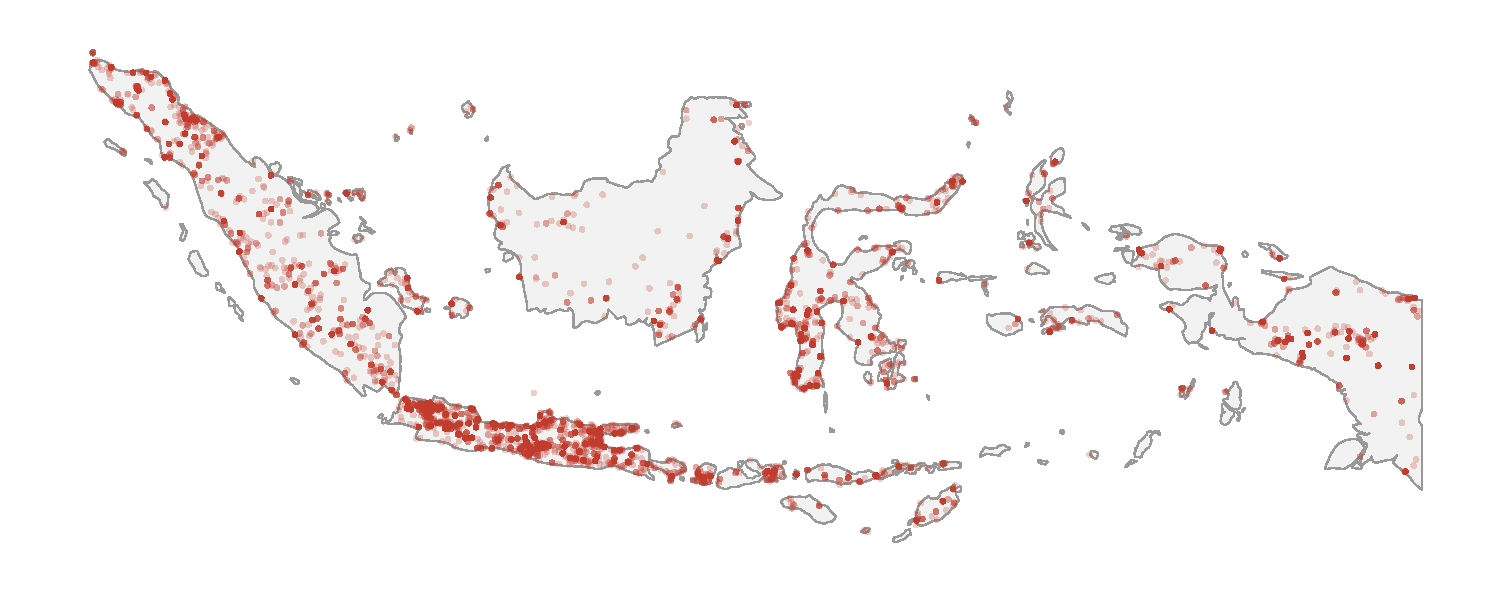
\includegraphics[width=0.95\textwidth]{figures/fig_spatial_distribution.pdf}
\end{center}

\vspace{-0.5em}
\begin{center}
\small
Protests concentrate in Java (center); sparse in eastern Indonesia
\end{center}

\end{frame}

% -----------------------------------------------------------------------------
\begin{frame}{Temporal Distribution}

\begin{center}
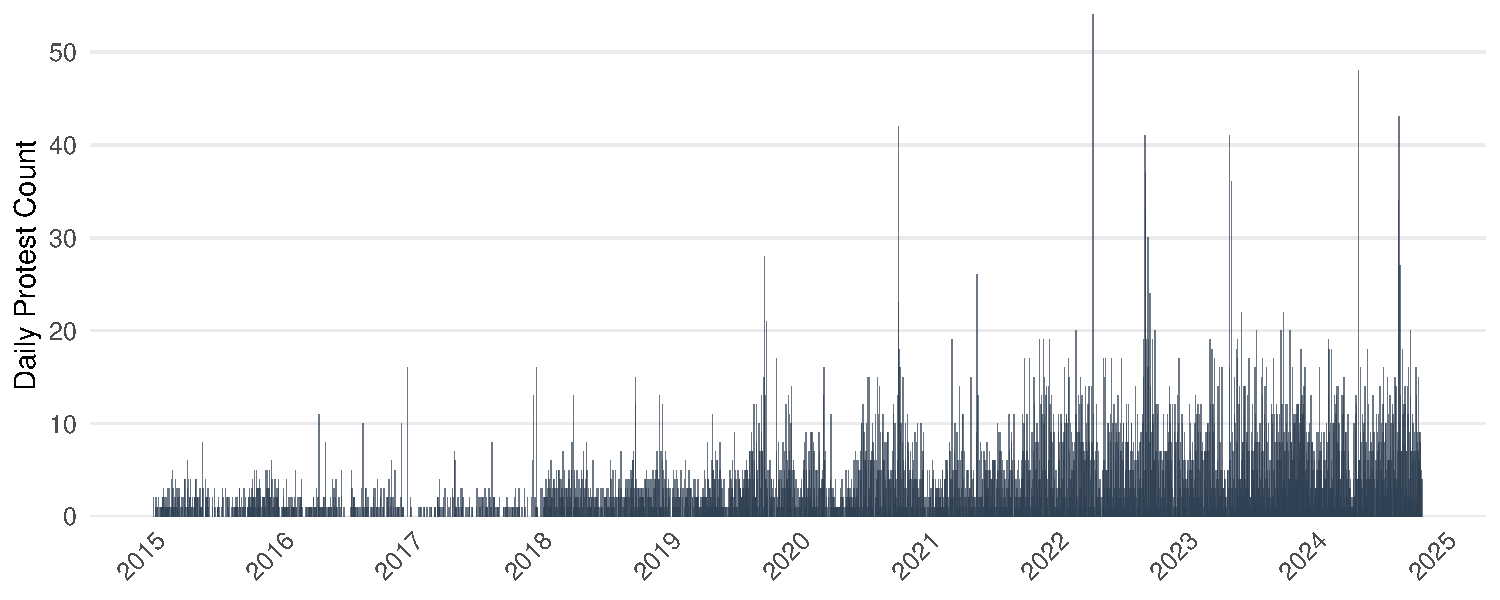
\includegraphics[width=0.95\textwidth]{figures/fig_timeseries.pdf}
\end{center}

\vspace{-0.5em}
\begin{center}
\small
Clustering and temporal bursts consistent with self-exciting dynamics
\end{center}

\end{frame}

% =============================================================================
% SECTION 4: RESULTS
% =============================================================================

\section{Results}

% -----------------------------------------------------------------------------
\begin{frame}{Test 1: Does Cross-District Contagion Exist?}

\begin{center}
\begin{tabular}{lcc}
\toprule
& \textbf{M0: Background} & \textbf{M1: + Contagion} \\
& \textbf{Only} & ($\theta = 100$ km) \\
\midrule
Deviance & 108,713 & 108,518 \\
Parameters & 13 & 14 \\
\bottomrule
\end{tabular}
\end{center}

\vspace{1em}

\textbf{F-test for nested models:}

\begin{equation*}
F = \frac{(D_0 - D_1)/1}{\phi} = \frac{(108713 - 108518)/1}{1.056} = 184.6
\end{equation*}

\vspace{0.5em}

\begin{center}
$F(1, 1{,}557{,}187) = 184.6$, \quad $p < 10^{-41}$
\end{center}

\vspace{0.5em}

\textbf{Result:} Strong evidence for cross-district contagion

\end{frame}

% -----------------------------------------------------------------------------
\begin{frame}{Coefficient Estimates}

\begin{center}
\small
\begin{tabular}{lcccc}
\toprule
& \textbf{Estimate} & \textbf{SE} & \textbf{$z$} & \textbf{$p$} \\
\midrule
Intercept & $-19.03$ & 0.902 & $-21.1$ & $<0.001$ \\
$\log(\text{population})$ & 0.636 & 0.012 & 54.5 & $<0.001$ \\
Poverty rate & $-0.021$ & 0.002 & $-11.7$ & $<0.001$ \\
CPI & 0.049 & 0.009 & 5.7 & $<0.001$ \\
\midrule
\textbf{Cross-district ($\alpha$)} & \textbf{0.323} & \textbf{0.023} & \textbf{14.0} & $<$\textbf{0.001} \\
\midrule
\multicolumn{5}{l}{\textit{Year fixed effects included (2016--2024)}} \\
\bottomrule
\multicolumn{5}{l}{Dispersion $\phi = 1.056$; $N = 1{,}557{,}200$ district-days} \\
\end{tabular}
\end{center}

\vspace{0.5em}

\textbf{Interpretation:} Multiplicative effect $\exp(\alpha) = 1.38$ per unit increase in cross-district exposure

\end{frame}

% -----------------------------------------------------------------------------
\begin{frame}{Magnitude: Branching Ratio and Endogenous Fraction}

\textbf{Branching ratio} (expected triggered events per original event):
\vspace{-0.5em}
\begin{equation*}
\text{BR} = \sum_s \sum_{\ell} E[\lambda_s] \cdot \left(\exp(\alpha \cdot w_{rs}) - 1\right) = 0.11
\end{equation*}
\vspace{-0.5em}
\begin{itemize}
    \item \textbf{Subcritical} (BR $< 1$): Process is stable, not explosive
    \item Each protest triggers $\approx 0.11$ additional protests elsewhere
\end{itemize}

\vspace{0.5em}

\textbf{Endogenous fraction} (share of events due to contagion):
\vspace{-0.5em}
\begin{equation*}
\frac{\sum_{t,r} \left(\hat{\lambda}_{t,r}^{\text{full}} - \hat{\lambda}_{t,r}^{\text{background}}\right)}{\sum_{t,r} \hat{\lambda}_{t,r}^{\text{full}}} = 14.4\%
\end{equation*}
\vspace{-0.5em}
\begin{itemize}
    \item $\sim$86\% driven by background (exogenous) factors
    \item $\sim$14\% attributable to cross-district contagion
\end{itemize}

\end{frame}

% -----------------------------------------------------------------------------
\begin{frame}{Test 2: Does Distance Matter?}

\textbf{Profile likelihood over $\theta$:}

\begin{center}
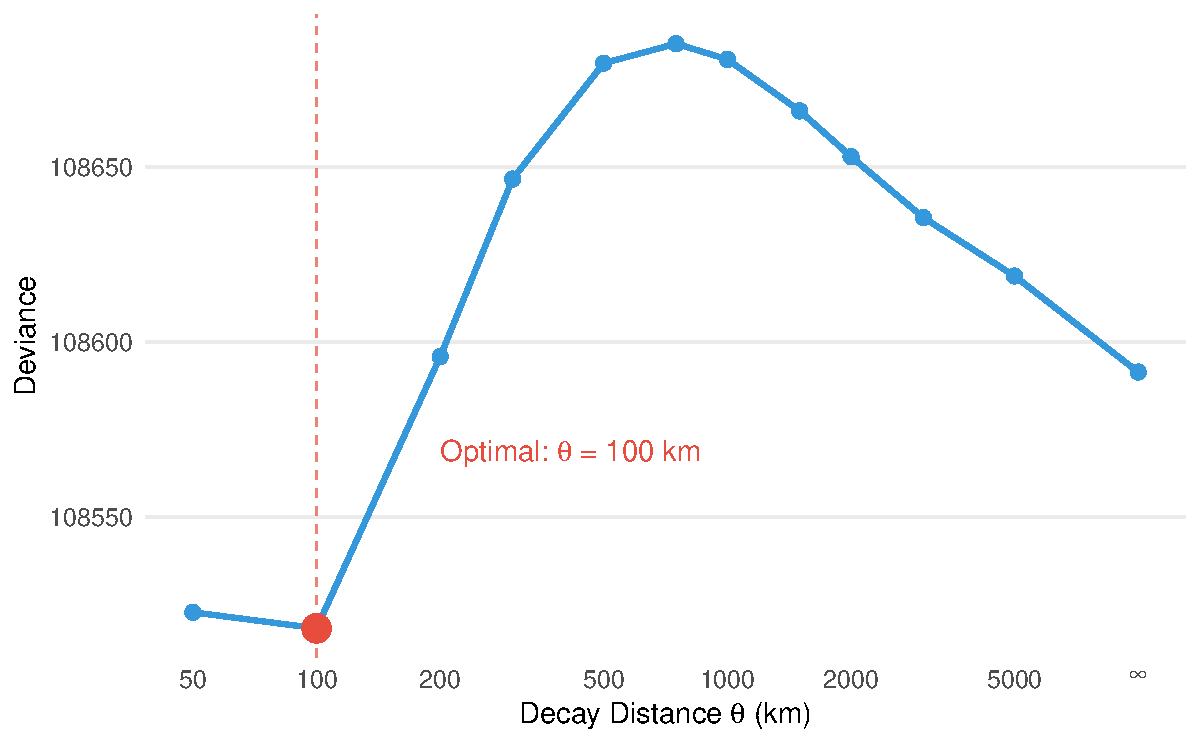
\includegraphics[width=0.75\textwidth]{figures/fig_profile_likelihood.pdf}
\end{center}

\vspace{-0.5em}

\textbf{Optimal:} $\hat{\theta} = 100$ km (deviance = 108,518)

\end{frame}

% -----------------------------------------------------------------------------
\begin{frame}{Test 2: Formal Hypothesis Test}

\textbf{Test:} $H_0: \theta = \infty$ vs $H_1: \theta < \infty$

\vspace{1em}

\begin{center}
\begin{tabular}{lcc}
\toprule
& $\theta = 100$ km & $\theta = \infty$ \\
\midrule
Deviance & 108,518 & 108,591 \\
$\hat{\alpha}$ & 0.323 & 1.022 \\
\bottomrule
\end{tabular}
\end{center}

\vspace{1em}

\textbf{Likelihood ratio test:}

\begin{equation*}
\text{LR} = \frac{D_{\infty} - D_{\hat{\theta}}}{\phi} = \frac{108591 - 108518}{1.056} = 69.1
\end{equation*}

\vspace{0.5em}

\begin{center}
$\chi^2(1) = 69.1$, \quad $p < 0.001$
\end{center}

\vspace{0.5em}

\textbf{Result:} Reject uniform weighting; distance decay is significant

\end{frame}

% -----------------------------------------------------------------------------
\begin{frame}{Conclusion}

\textbf{Findings:}

\begin{enumerate}
    \item \textbf{Recent protests elsewhere predict protests today}
    \begin{itemize}
        \item Protests in other districts over past 30 days $\rightarrow$ more protests here
        \item $F(1, 1.56\text{M}) = 185$, $p < 10^{-41}$
    \end{itemize}

    \vspace{0.3em}

    \item \textbf{Effect is local, not national}
    \begin{itemize}
        \item $\hat{\theta} = 100$ km; influence decays with distance
        \item Reject uniform national spread ($p < 0.001$)
    \end{itemize}

    \vspace{0.3em}

    \item \textbf{Effect is modest but significant}
    \begin{itemize}
        \item BR $= 0.11$ (subcritical); 14\% triggered by cross-district contagion
    \end{itemize}
\end{enumerate}

\vspace{0.5em}

\textbf{Contribution:} Discrete spatial-temporal Hawkes model; distinguishes local vs.\ national diffusion

\end{frame}

% -----------------------------------------------------------------------------
\begin{frame}{Next Steps: Violent vs.\ Non-Violent Events}

\textbf{Question:} Do violent and non-violent events have different mobilization potential?

\vspace{1em}

\textbf{Approach:}
\begin{itemize}
    \item Separate events by type (protests vs.\ riots/violence)
    \item Estimate cross-type contagion effects:
    \begin{itemize}
        \item Do non-violent protests trigger more protests?
        \item Do violent events trigger more violence---or suppress mobilization?
    \end{itemize}
    \item Compare branching ratios across event types
\end{itemize}

\vspace{1em}

\textbf{Why it matters:}
\begin{itemize}
    \item Informs debate on tactical choice in social movements
    \item Tests whether violence escalates or dampens collective action
\end{itemize}

\end{frame}

% -----------------------------------------------------------------------------
\begin{frame}[standout]
    Thank You

    \vspace{1em}

    \normalsize
    Questions?
\end{frame}

% =============================================================================
% APPENDIX
% =============================================================================

\appendix

% -----------------------------------------------------------------------------
\begin{frame}{Appendix: Temporal Lag Structure}

\textbf{Model with weekly lag bins} ($\theta = 100$ km):

\begin{center}
\small
\begin{tabular}{lcccc}
\toprule
& \textbf{Estimate} & \textbf{SE} & \textbf{$t$} & \textbf{$p$} \\
\midrule
Week 1 (lags 1--7) & 4.28 & 0.25 & 17.0 & $<0.001$ \\
Week 2 (lags 8--14) & 0.49 & 0.29 & 1.7 & 0.091 \\
Week 3 (lags 15--21) & 0.24 & 0.30 & 0.8 & 0.421 \\
Week 4 (lags 22--30) & $-0.42$ & 0.24 & $-1.7$ & 0.086 \\
\bottomrule
\end{tabular}
\end{center}

\vspace{0.5em}
\begin{center}
\small
Effect concentrated in Week 1; fades rapidly thereafter
\end{center}

\end{frame}

% -----------------------------------------------------------------------------
\begin{frame}{Appendix: Covariate Effects}

\begin{center}
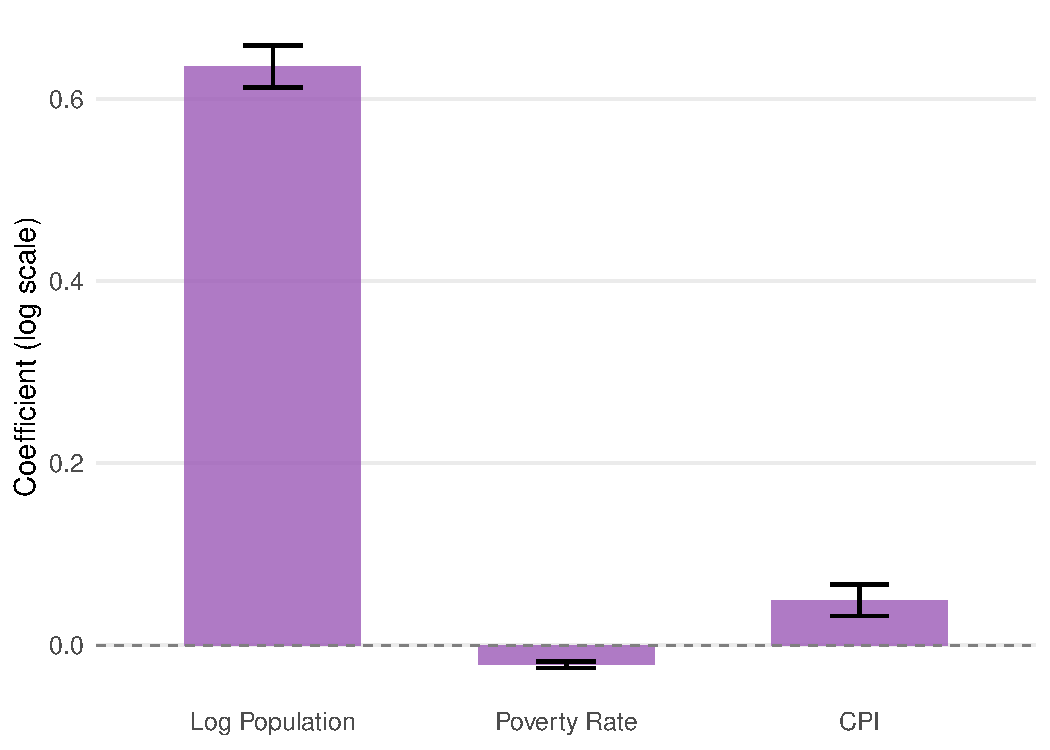
\includegraphics[width=0.75\textwidth]{figures/fig_covariates.pdf}
\end{center}

\vspace{-0.5em}
\begin{center}
\small
Background rate: Population (+), CPI/Inflation (+), Poverty ($-$)
\end{center}

\end{frame}

% -----------------------------------------------------------------------------
\begin{frame}{Appendix: Profile Likelihood Detail}

\begin{center}
\small
\begin{tabular}{rcccc}
\toprule
$\theta$ (km) & Deviance & $\hat{\alpha}$ & SE($\hat{\alpha}$) & $t$ \\
\midrule
50 & 108,523 & 0.229 & 0.016 & 13.9 \\
\textbf{100} & \textbf{108,518} & \textbf{0.323} & \textbf{0.023} & \textbf{14.0} \\
200 & 108,596 & 0.385 & 0.036 & 10.7 \\
300 & 108,647 & 0.368 & 0.047 & 7.9 \\
500 & 108,680 & 0.336 & 0.060 & 5.6 \\
1000 & 108,681 & 0.420 & 0.076 & 5.5 \\
2000 & 108,653 & 0.645 & 0.086 & 7.5 \\
$\infty$ & 108,591 & 1.022 & 0.095 & 10.7 \\
\bottomrule
\end{tabular}
\end{center}

\vspace{0.5em}

\textbf{Note:} Minimum deviance at $\theta = 100$ km

\end{frame}

\end{document}
